\chapter{Image formation}

\section{Camera and lens}

    \subsection{Image formation}
    \begin{enumerate}
        \item Pinhole camera: \transtip{光圈}{aperture}(小孔成像), 过小会发生衍射, 且通光量过少.
        \item Lens: 汇聚光线, $\frac{1}{i}+\frac{1}{o}=\frac{1}{f}$, 可用平行光测量$f$, \transtip{放大率}{Magnification}: $m=\frac{h_i}{h_o}=\frac{i}{o}$, 现阶段\transtip{像距}{i}基本上等于\transtip{焦距}{f}, 同时焦距也决定了视野.
        \begin{figure}[H]
            \begin{subfigure}{0.33\textwidth}
                    \centering
                    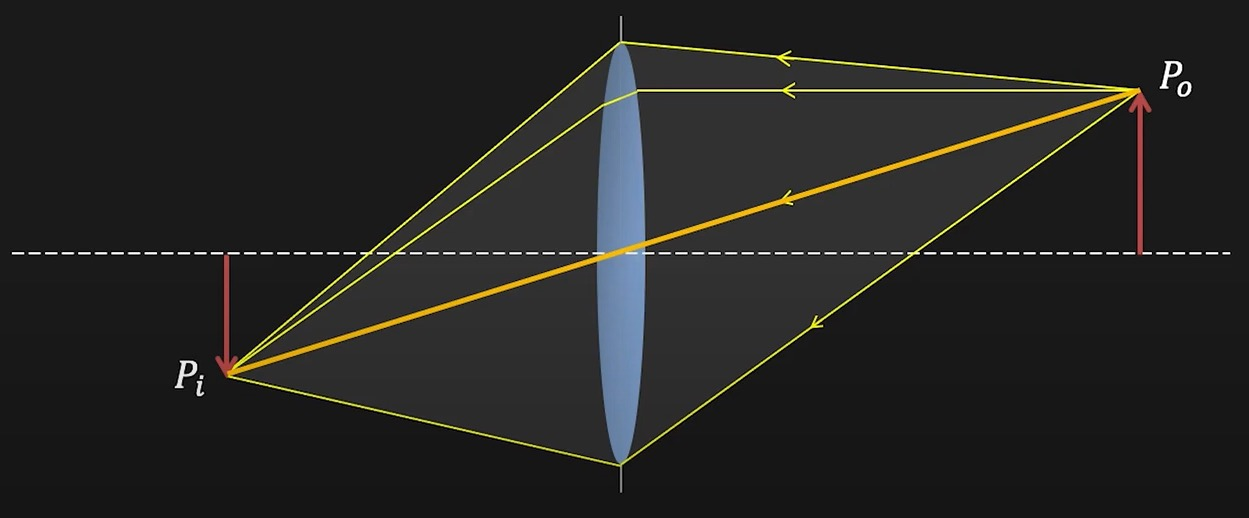
\includegraphics[width=\textwidth]{/Lec2/Lens}
                    \caption{Lens}
            \end{subfigure}
            \begin{subfigure}{0.33\textwidth}
                \centering
                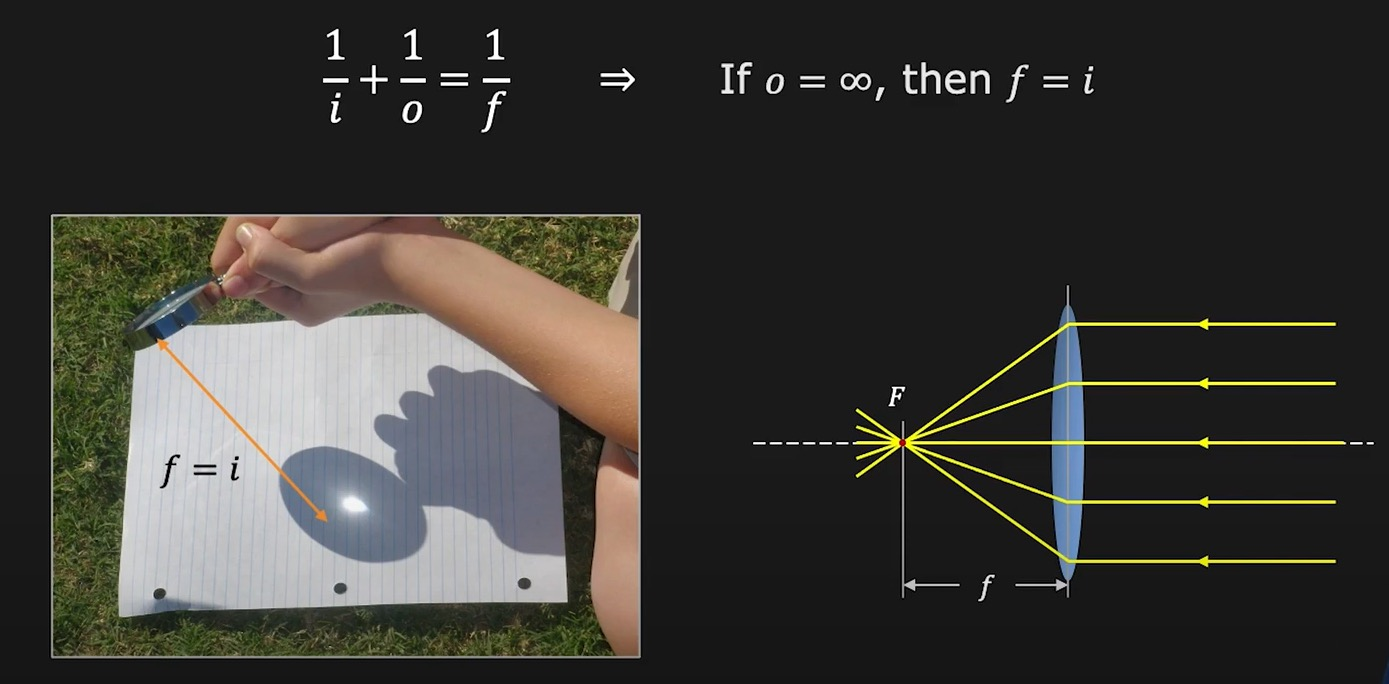
\includegraphics[width=\textwidth]{/Lec2/Focal}
                \caption{f}
            \end{subfigure}
            \begin{subfigure}{0.33\textwidth}
                \centering
                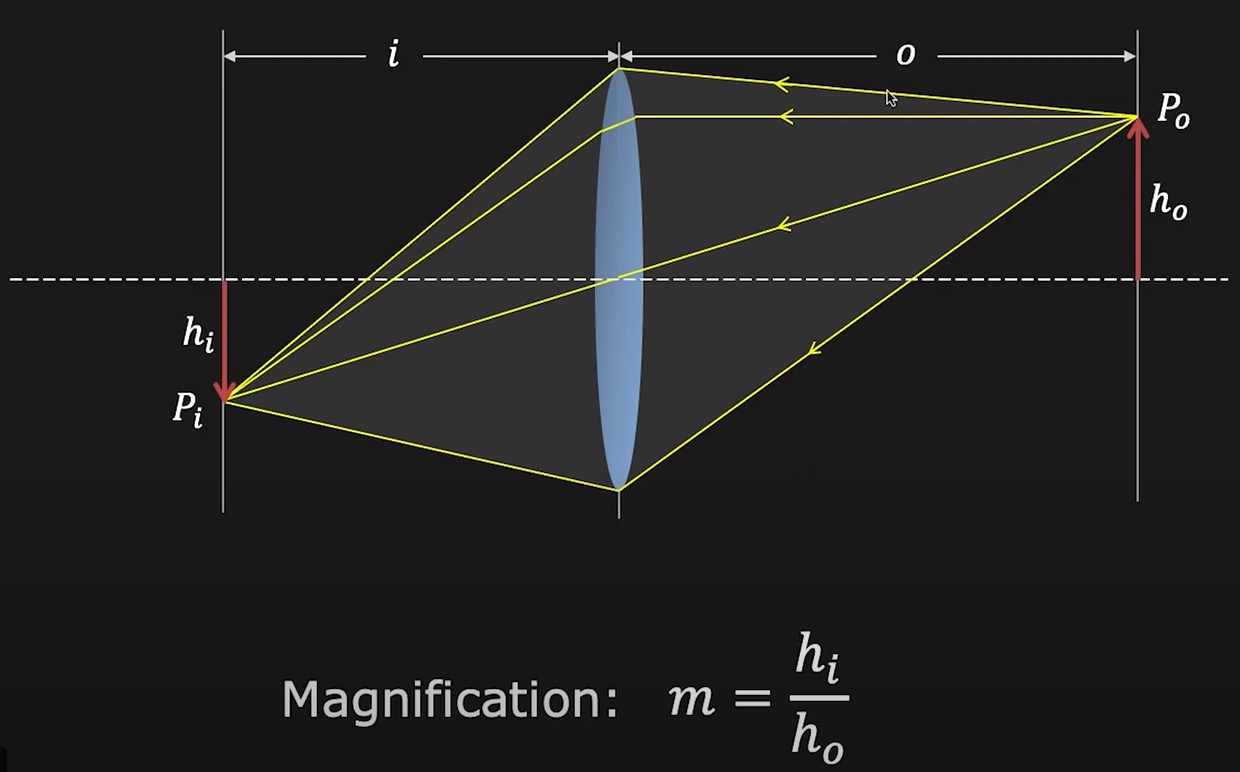
\includegraphics[width=\textwidth]{/Lec2/Magnification}
                \caption{Magnification}
            \end{subfigure}
            \caption{Lens}
        \end{figure}
        \item \transtip{视野}{Field of View}(FOV), 不同焦距也影响着背景的变化
        \begin{figure}[H]
            \begin{subfigure}{0.33\textwidth}
                \centering
                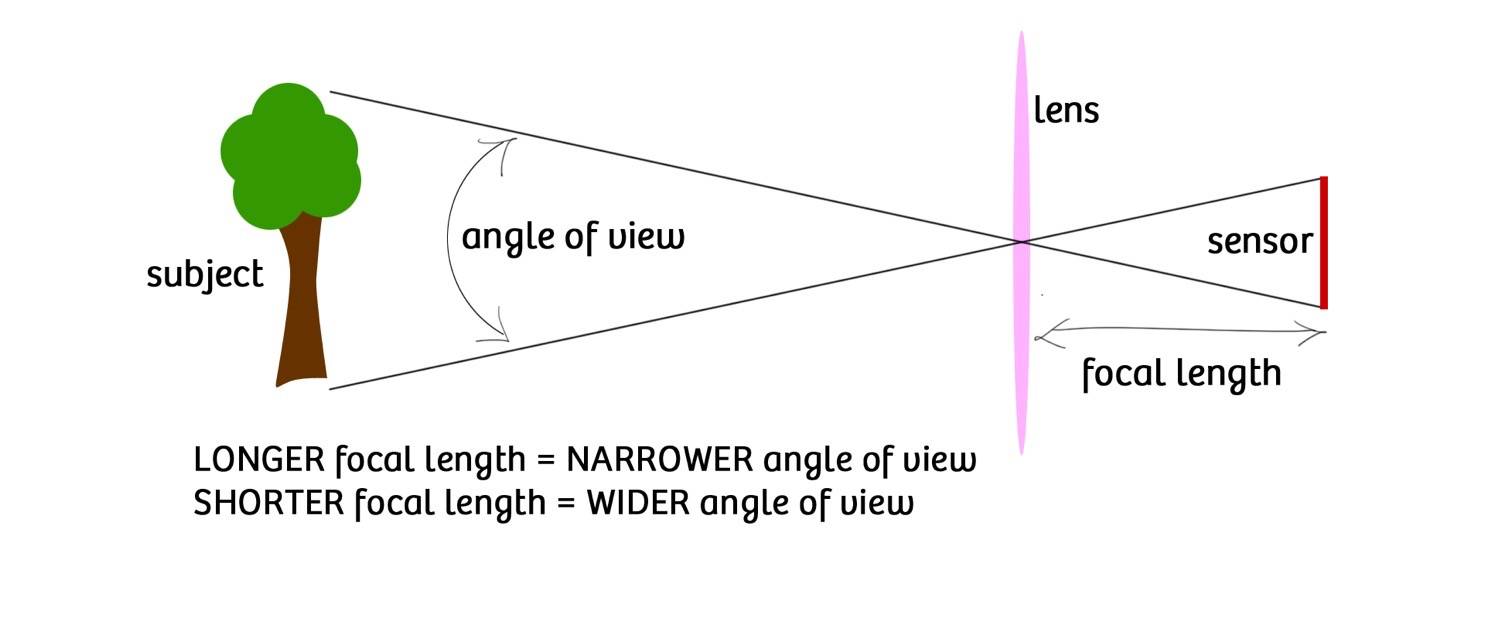
\includegraphics[width=\textwidth]{/Lec2/FOV}
                \caption{FOV}
            \end{subfigure}
            \begin{subfigure}{0.33\textwidth}
                \centering
                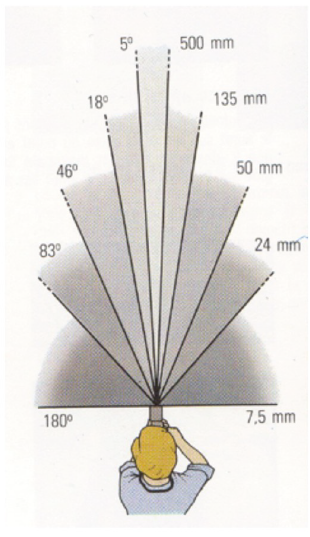
\includegraphics[width=0.5\textwidth]{/Lec2/FFOV}
                \caption{焦距与视野}
            \end{subfigure}
            \begin{subfigure}{0.33\textwidth}
                \centering
                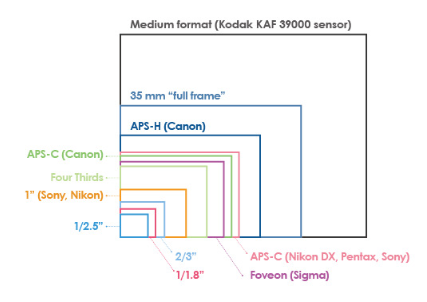
\includegraphics[width=\textwidth]{/Lec2/sensor}
                \caption{镜头与视野}
            \end{subfigure}
            \caption{FOV}
        \end{figure}
        \item Aperture: $D=\frac{f}{N}$, N is called \transtip{F数}{F-Number}.
        \item Lens \transtip{散焦}{defocus}, 会成斑. 
        \begin{align*}
            b=\frac{D}{i'}\left|i'-i\right|, b\varpropto D \varpropto \frac{1}{N}
        \end{align*}
        b是斑的大小.
        \begin{figure}[H]
            \centering
            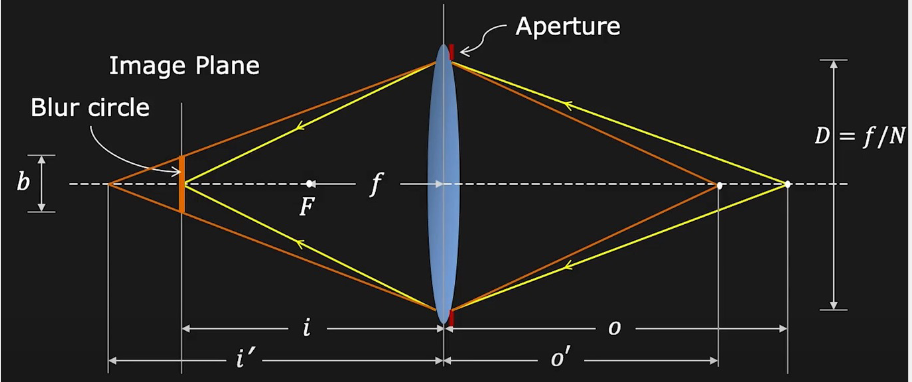
\includegraphics[width=0.38\textwidth]{/Lec2/Lens defocus}
            \caption{Lens defocus}
        \end{figure}
        \item \transtip{对焦}{Focusing}
        \item \transtip{景深}{Depth of Field}(DOF)
        \begin{align*}
            c&=\frac{f^2(o-o_1)}{No_1(o-f)}\\
            c&=\frac{f^2(o_2-o)}{No_2(o-f)}\\
            (DOF)o_2-o_1&=\frac{2of^2cN(o-f)}{f^4-c^2N^2(o-f)^2}
        \end{align*}
        \begin{figure}[H]
            \centering
            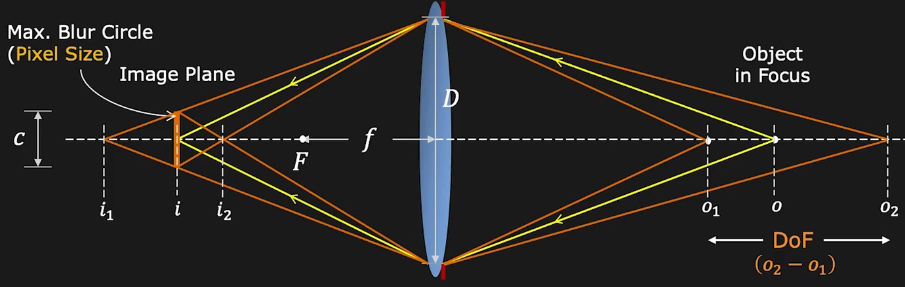
\includegraphics[width=0.38\textwidth]{/Lec2/DOF}
            \caption{DOF}
        \end{figure}

        To \transtip{虚化背景}{blur the background}:\begin{enumerate}
            \item Large aperture
            \item Long focal length
            \item Near foreground
            \item Far Background
        \end{enumerate}
    \end{enumerate}

\section{Geometric image formation}
\transtip{相机模型}{Camera model} describes the geometric relation between 3D world and 2D image

\subsection{Pin-hole camera model}
\begin{enumerate}
    \item \transtip{透视变换}{Perspective Projection}
    \begin{figure}[H]
        \centering
        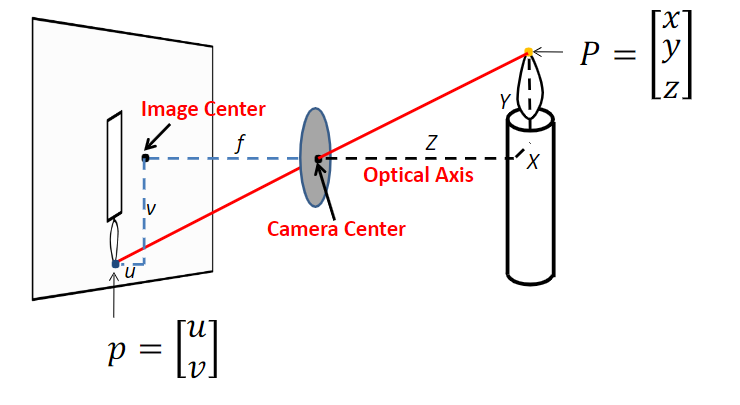
\includegraphics[width=0.38\textwidth]{/Lec2/Pin-hole}
        \caption{Pin-hole}
    \end{figure}
    \begin{align*}
        p=\begin{bmatrix}
            u\\v
        \end{bmatrix}=\begin{bmatrix}
            f\frac{x}{z}\\ f\frac{y}{z}
        \end{bmatrix}
    \end{align*}
    
    \item \transtip{齐次坐标}{Homogeneous coordinates}
    
    Also called projective coordinates.

    \begin{align*}
        \begin{bmatrix}
            f&0&0&0\\
            0&f&0&0\\
            0&0&1&0
        \end{bmatrix}\begin{bmatrix}
            x\\y\\z\\1
        \end{bmatrix}=\begin{bmatrix}
            fx\\fy\\z
        \end{bmatrix}\cong \begin{bmatrix}
            f\frac{x}{z}\\f\frac{y}{z}\\1
        \end{bmatrix}
    \end{align*}
    \begin{figure}[H]
        \centering
        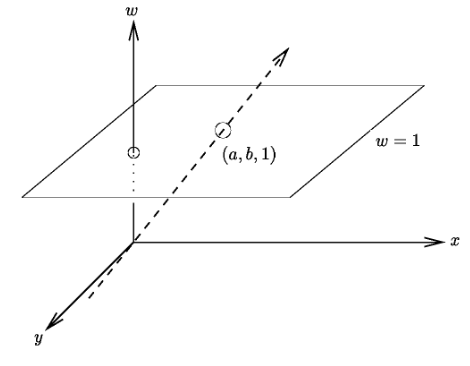
\includegraphics[width=0.38\textwidth]{/Lec2/coordinate}
        \caption{Homogeneous coordinates}
    \end{figure}
    将二维的点升维到三维过原点的射线. 二维的平移可以等效于三维的旋转. 
    \item Visualize Perspective Projection
    \begin{figure}[H]
        \centering
        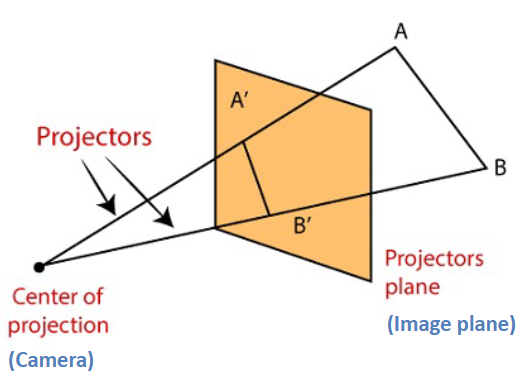
\includegraphics[width=0.38\textwidth]{/Lec2/VPP}
        \caption{Perspective Projection}
    \end{figure}
    \item 信息损失
    \begin{enumerate}
        \item 深度
        \item 长度(因为损失深度)
        \item 角度
        \item 非双射, 一个二平面可以对应无数三维物体
    \end{enumerate}
    \item 信息保留
    \begin{enumerate}
        \item 线性: 直线还是直线
    \end{enumerate}
    \item \transtip{灭点}{Vanishing points}
    
    一组平行的线的交点, 可以在画外or无穷远处
    \begin{figure}[H]
        \centering
        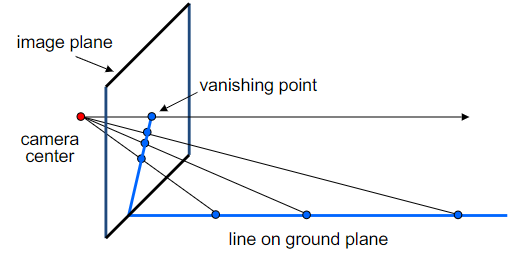
\includegraphics[width=0.38\textwidth]{/Lec2/vanishing point}
        \caption{Vanishing points}
    \end{figure}

    Properties:
    \begin{enumerate}
        \item 任意两条平行线会交于一个灭点
        \item \transtip{camera center}{C} \transtip{vanishing point}{V} 平行于三维的线
    \end{enumerate}

    可以获得平行线的朝向or相机的朝向
    
    \item \transtip{地平线}{Vanishing lines}
    
    一个平面内所有平行线的灭点的连线, 地平线与相机中心构成的平面与原平面平行. 

    \item Perspective \transtip{畸变}{distortion}
    \begin{figure}[H]
        \centering
        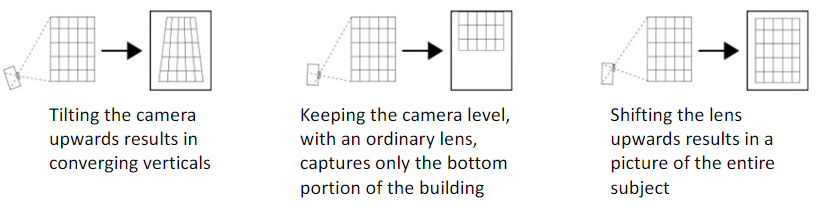
\includegraphics[width=0.5\textwidth]{/Lec2/distortion}
        \caption{Perspective distortion}
    \end{figure}

    解决方案: 移轴镜头

    越边界越大, 不是因为镜头
    \begin{figure}[H]
        \centering
        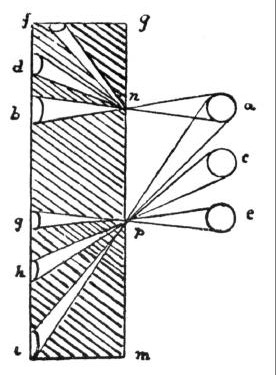
\includegraphics[width=0.12\textwidth]{/Lec2/pdd}
        \caption{Perspective distortion}
    \end{figure}
    \item Distortion
    
    是因为镜头造成的, 可以后期矫正的
    \begin{figure}[H]
        \centering
        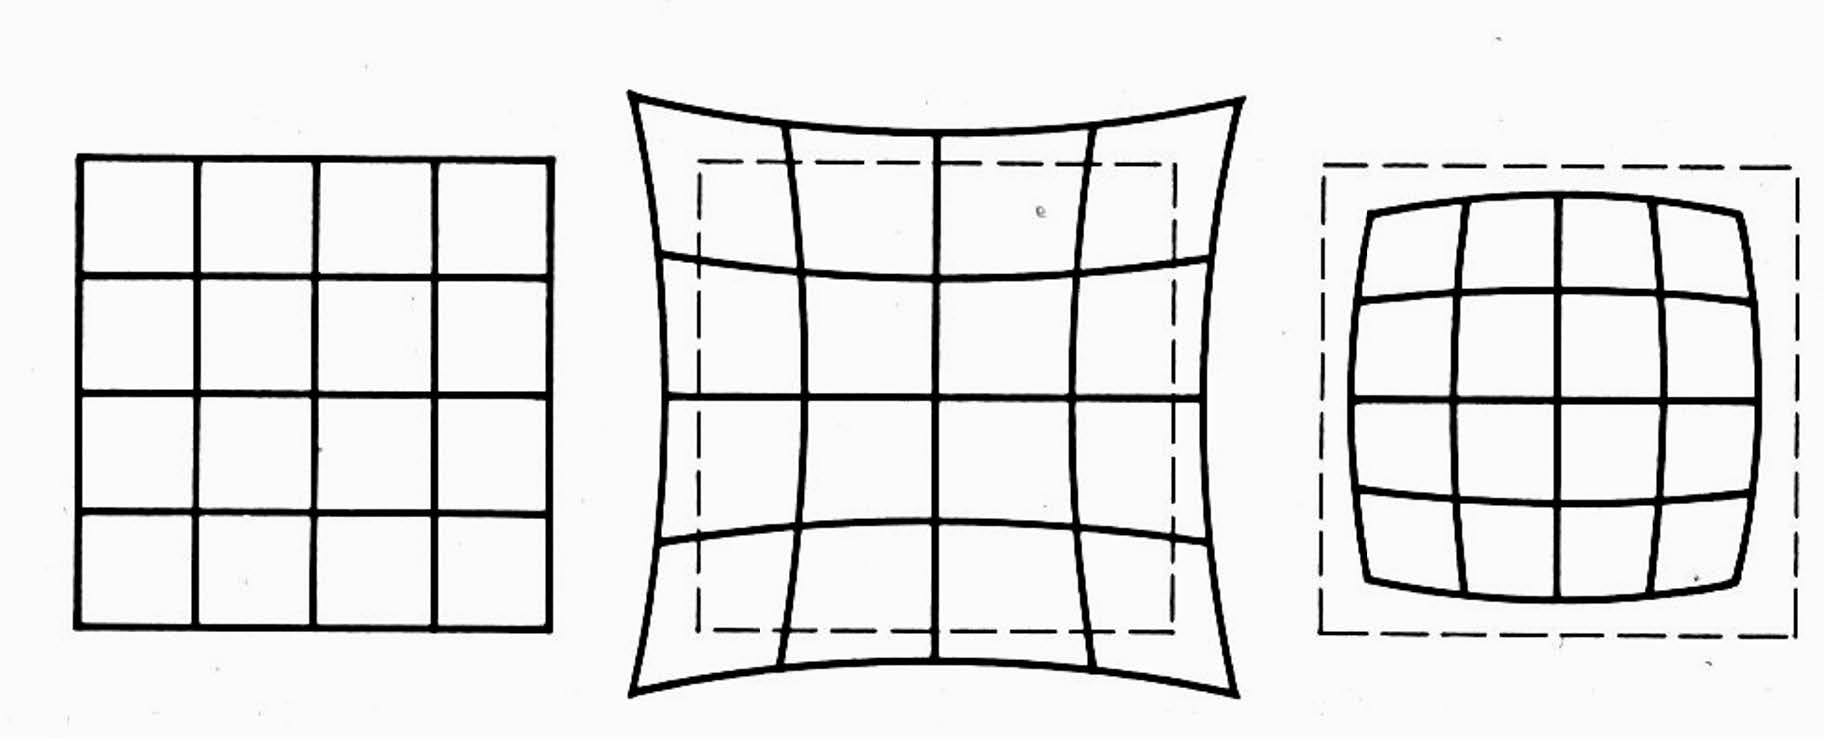
\includegraphics[width=0.38\textwidth]{/Lec2/dd}
        \caption{无畸变,枕形畸变,筒形畸变}
    \end{figure}
    \begin{align*}
        r^2&={x'}_n^2+{y'}_n^2\\
        {x'}_d&={x'}_n(1+k_1r^2+k_2r^4)\\
        {y'}_d&={y'}_n(1+k_1r^2+k_2r^4)
    \end{align*}
\end{enumerate}
\subsection{Orthographic projection}
正交投影, 简单但不符合实际, 只是种近似. 

\begin{figure}[H]
    \centering
    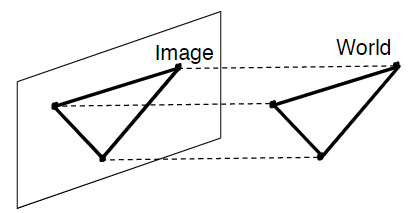
\includegraphics[width=0.38\textwidth]{/Lec2/orthographic}
    \caption{正交投影}
\end{figure}

\begin{align*}
    \begin{bmatrix}
        1&0&0&0\\0&1&0&0\\0&0&0&1
    \end{bmatrix}\begin{bmatrix}
        x\\y\\z\\1
    \end{bmatrix}=\begin{bmatrix}
        x\\y\\1
    \end{bmatrix}\Rightarrow (x,y)
\end{align*}

\section{Photometric image formation}

\subsection{Image sensor}
每个像素是光强关于时间的积分.
\begin{enumerate}
    \item CMOS(Complimentary Metal-Oxide
    Semiconductor): 数码底片, 光->电, 进行记录
    \item CCD(Charge Coupled Device): 用的少了
\end{enumerate}

\subsection{Shutter}
\begin{figure}[H]
    \centering
    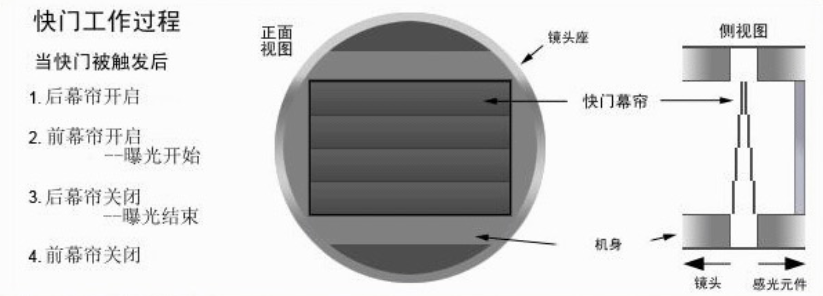
\includegraphics[width=0.38\textwidth]{/Lec2/shutter}
    \caption{快门}
\end{figure}
\begin{enumerate}
    \item Shutter speed: 快门/曝光时间
    \item Shutter effect: 不同曝光时间的效应
    \item IOS: 传感器敏感度
    \item rolling shutter effect: 快门一行一行打开, 导致物体结构被破坏了
\end{enumerate}

\subsection{Color sensing in camera}
颜色和波长有关
\begin{enumerate}
    \item Color spaces: RGB(所有颜色是由R,G,B混合而成), HSV(\transtip{色调}{Hue}, \transtip{饱和度}{Saturation}, value)
    \item \transtip{贝尔滤波器}{Bayer filter}
    \begin{figure}[H]
        \centering
        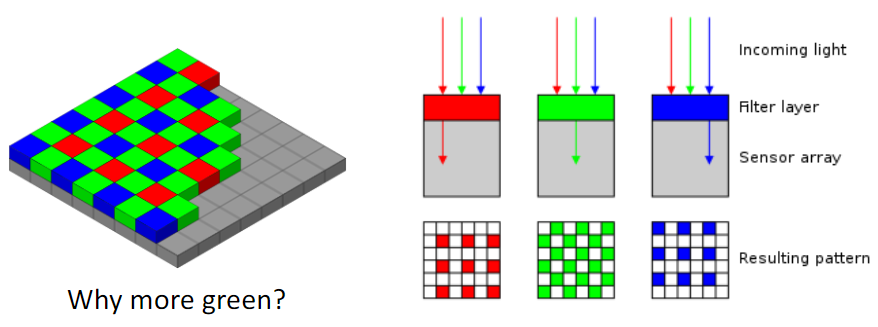
\includegraphics[width=0.38\textwidth]{/Lec2/Bayer}
        \caption{Bayer filter}
    \end{figure}
    旁边颜色用插值获取, 绿色多因为人眼对绿光更敏感, 绿光多信噪比更好. 
\end{enumerate}

